\documentclass[aspectratio=169,10pt]{beamer}

\usepackage{graphicx}
\usepackage{booktabs}
\usepackage{array}
\usepackage{amsmath}
\usepackage{hyperref}

\definecolor{Ink}{HTML}{111827}
\definecolor{Muted}{HTML}{4B5563}
\definecolor{Accent}{HTML}{0F766E}
\definecolor{AccentLight}{HTML}{E6FFFB}
\definecolor{Rule}{HTML}{D1D5DB}

\usetheme{default}
\usefonttheme{professionalfonts}
\setbeamertemplate{navigation symbols}{}
\setbeamertemplate{caption}[numbered]
\setbeamertemplate{footline}{%
  \leavevmode%
  \hbox{%
    \begin{beamercolorbox}[wd=.72\paperwidth,ht=2.4ex,dp=1.0ex,leftskip=1.2em]{author in head/foot}%
      \usebeamerfont{author in head/foot}\insertshorttitle
    \end{beamercolorbox}%
    \begin{beamercolorbox}[wd=.28\paperwidth,ht=2.4ex,dp=1.0ex,rightskip=1.2em plus1fil]{date in head/foot}%
      \usebeamerfont{date in head/foot}\hfill\insertframenumber/\inserttotalframenumber
    \end{beamercolorbox}}%
}
\setbeamercolor{normal text}{fg=Ink,bg=white}
\setbeamercolor{frametitle}{fg=Ink,bg=white}
\setbeamercolor{title}{fg=Ink,bg=white}
\setbeamercolor{structure}{fg=Accent}
\setbeamercolor{author in head/foot}{fg=Muted,bg=white}
\setbeamercolor{date in head/foot}{fg=Muted,bg=white}
\setbeamerfont{title}{series=\bfseries,size=\Large}
\setbeamerfont{frametitle}{series=\bfseries,size=\large}
\setbeamerfont{caption}{size=\scriptsize}
\setbeamertemplate{itemize item}{\color{Accent}$\blacktriangleright$}
\setbeamertemplate{itemize subitem}{\color{Accent}$\circ$}

\newcommand{\method}{RidgeLoRA-FP}
\newcommand{\smallnote}[1]{\par\vspace{0.35em}{\scriptsize\color{Muted}#1\par}}
\newcommand{\key}[1]{\textcolor{Accent}{\textbf{#1}}}

\title[Lightweight Cross-Sensor Fingerprint Generation]{Lightweight Cross-Sensor Fingerprint Generation\\via Ridge-Conditioned Diffusion}
\author[Nguyen, Pham, Nguyen]{Thanh Lam Nguyen\texorpdfstring{$^{*}$}{*}
  \and Chi Bang Pham\texorpdfstring{$^{*}$}{*}
  \and Phu An Nguyen\texorpdfstring{$^{*}$}{*}}
\institute{Hanoi University of Science and Technology\\
{\small $^{*}$Equal contribution \quad Supervisor: Dr. Tran Nguyen Ngoc}}
\date{Computer Vision Final Project}

\begin{document}

\begin{frame}[plain]
  \centering
  \vspace{1.0cm}
  {\usebeamerfont{title}\inserttitle\par}
  \vspace{0.35cm}
  {\color{Accent}\rule{0.62\linewidth}{0.7pt}\par}
  \vspace{0.9cm}
  {\normalsize Thanh Lam Nguyen\texorpdfstring{$^{*}$}{*}
  \hspace{1.6em} Chi Bang Pham\texorpdfstring{$^{*}$}{*}
  \hspace{1.6em} Phu An Nguyen\texorpdfstring{$^{*}$}{*}\par}
  \vspace{0.45cm}
  {\small Hanoi University of Science and Technology\par}
  \vspace{0.18cm}
  {\small \texorpdfstring{$^{*}$}{*}Equal contribution\par}
  \vspace{0.18cm}
  {\small Supervisor: Dr. Tran Nguyen Ngoc\par}
  \vfill
  {\small Computer Vision Final Project\par}
  \vspace{0.5cm}
\end{frame}

\begin{frame}{15-Minute Talk Map}
  \begin{columns}[T,onlytextwidth]
    \begin{column}{0.48\textwidth}
      \begin{block}{Core story}
        \begin{itemize}
          \item 2 min: problem and target-sensor setting
          \item 5 min: two-stage ridge-conditioned method
          \item 5 min: SD302A and FVC experiments
          \item 2 min: ablation, efficiency, limitations
          \item 1 min: conclusion and takeaways
        \end{itemize}
      \end{block}
    \end{column}
    \begin{column}{0.48\textwidth}
      \begin{block}{One-sentence thesis}
        Generate new fingerprint identities first, then render them into a
        target sensor style using explicit ridge control, target pose masks,
        and a tiny Stage-2 LoRA adapter.
      \end{block}
      \smallnote{Main metric throughout: verification TAR at FAR = 0.1\%.}
    \end{column}
  \end{columns}
\end{frame}

\begin{frame}{Problem: New Sensors Need Data}
  \begin{columns}[T,onlytextwidth]
    \begin{column}{0.56\textwidth}
      \begin{itemize}
        \item Fingerprint recognizers need many identities and repeated
        impressions per identity.
        \item Real biometric data is expensive, privacy-sensitive, and hard to
        share.
        \item A new deployed sensor may have only a small calibration set.
        \item Synthetic data must preserve \key{identity ridges/minutiae} while
        changing \key{sensor appearance, pose, mask, contrast, and artifacts}.
      \end{itemize}
    \end{column}
    \begin{column}{0.40\textwidth}
      \begin{block}{Target-sensor augmentation}
        Input: limited target-sensor samples.

        Output: many realistic training impressions that match that sensor
        without copying real identities.
      \end{block}
    \end{column}
  \end{columns}
\end{frame}

\begin{frame}{Key Idea and Contributions}
  \begin{columns}[T,onlytextwidth]
    \begin{column}{0.50\textwidth}
      \begin{block}{Design principle}
        Separate what must stay fixed from what should change.
      \end{block}
      \begin{itemize}
        \item Identity: ridge flow, ridge frequency, minutiae layout.
        \item Sensor domain: foreground footprint, gray tone, background,
        pressure/crop artifacts.
      \end{itemize}
    \end{column}
    \begin{column}{0.47\textwidth}
      \begin{block}{Contributions}
        \begin{itemize}
          \item Compact two-stage latent diffusion pipeline.
          \item Explicit Sauvola ridge condition for identity preservation.
          \item Stage-2 middle-attention LoRA for new sensor styles.
          \item Recognition, LightGlue, t-SNE, and ablation diagnostics.
        \end{itemize}
      \end{block}
    \end{column}
  \end{columns}
\end{frame}

\begin{frame}{Method Overview}
  \centering
  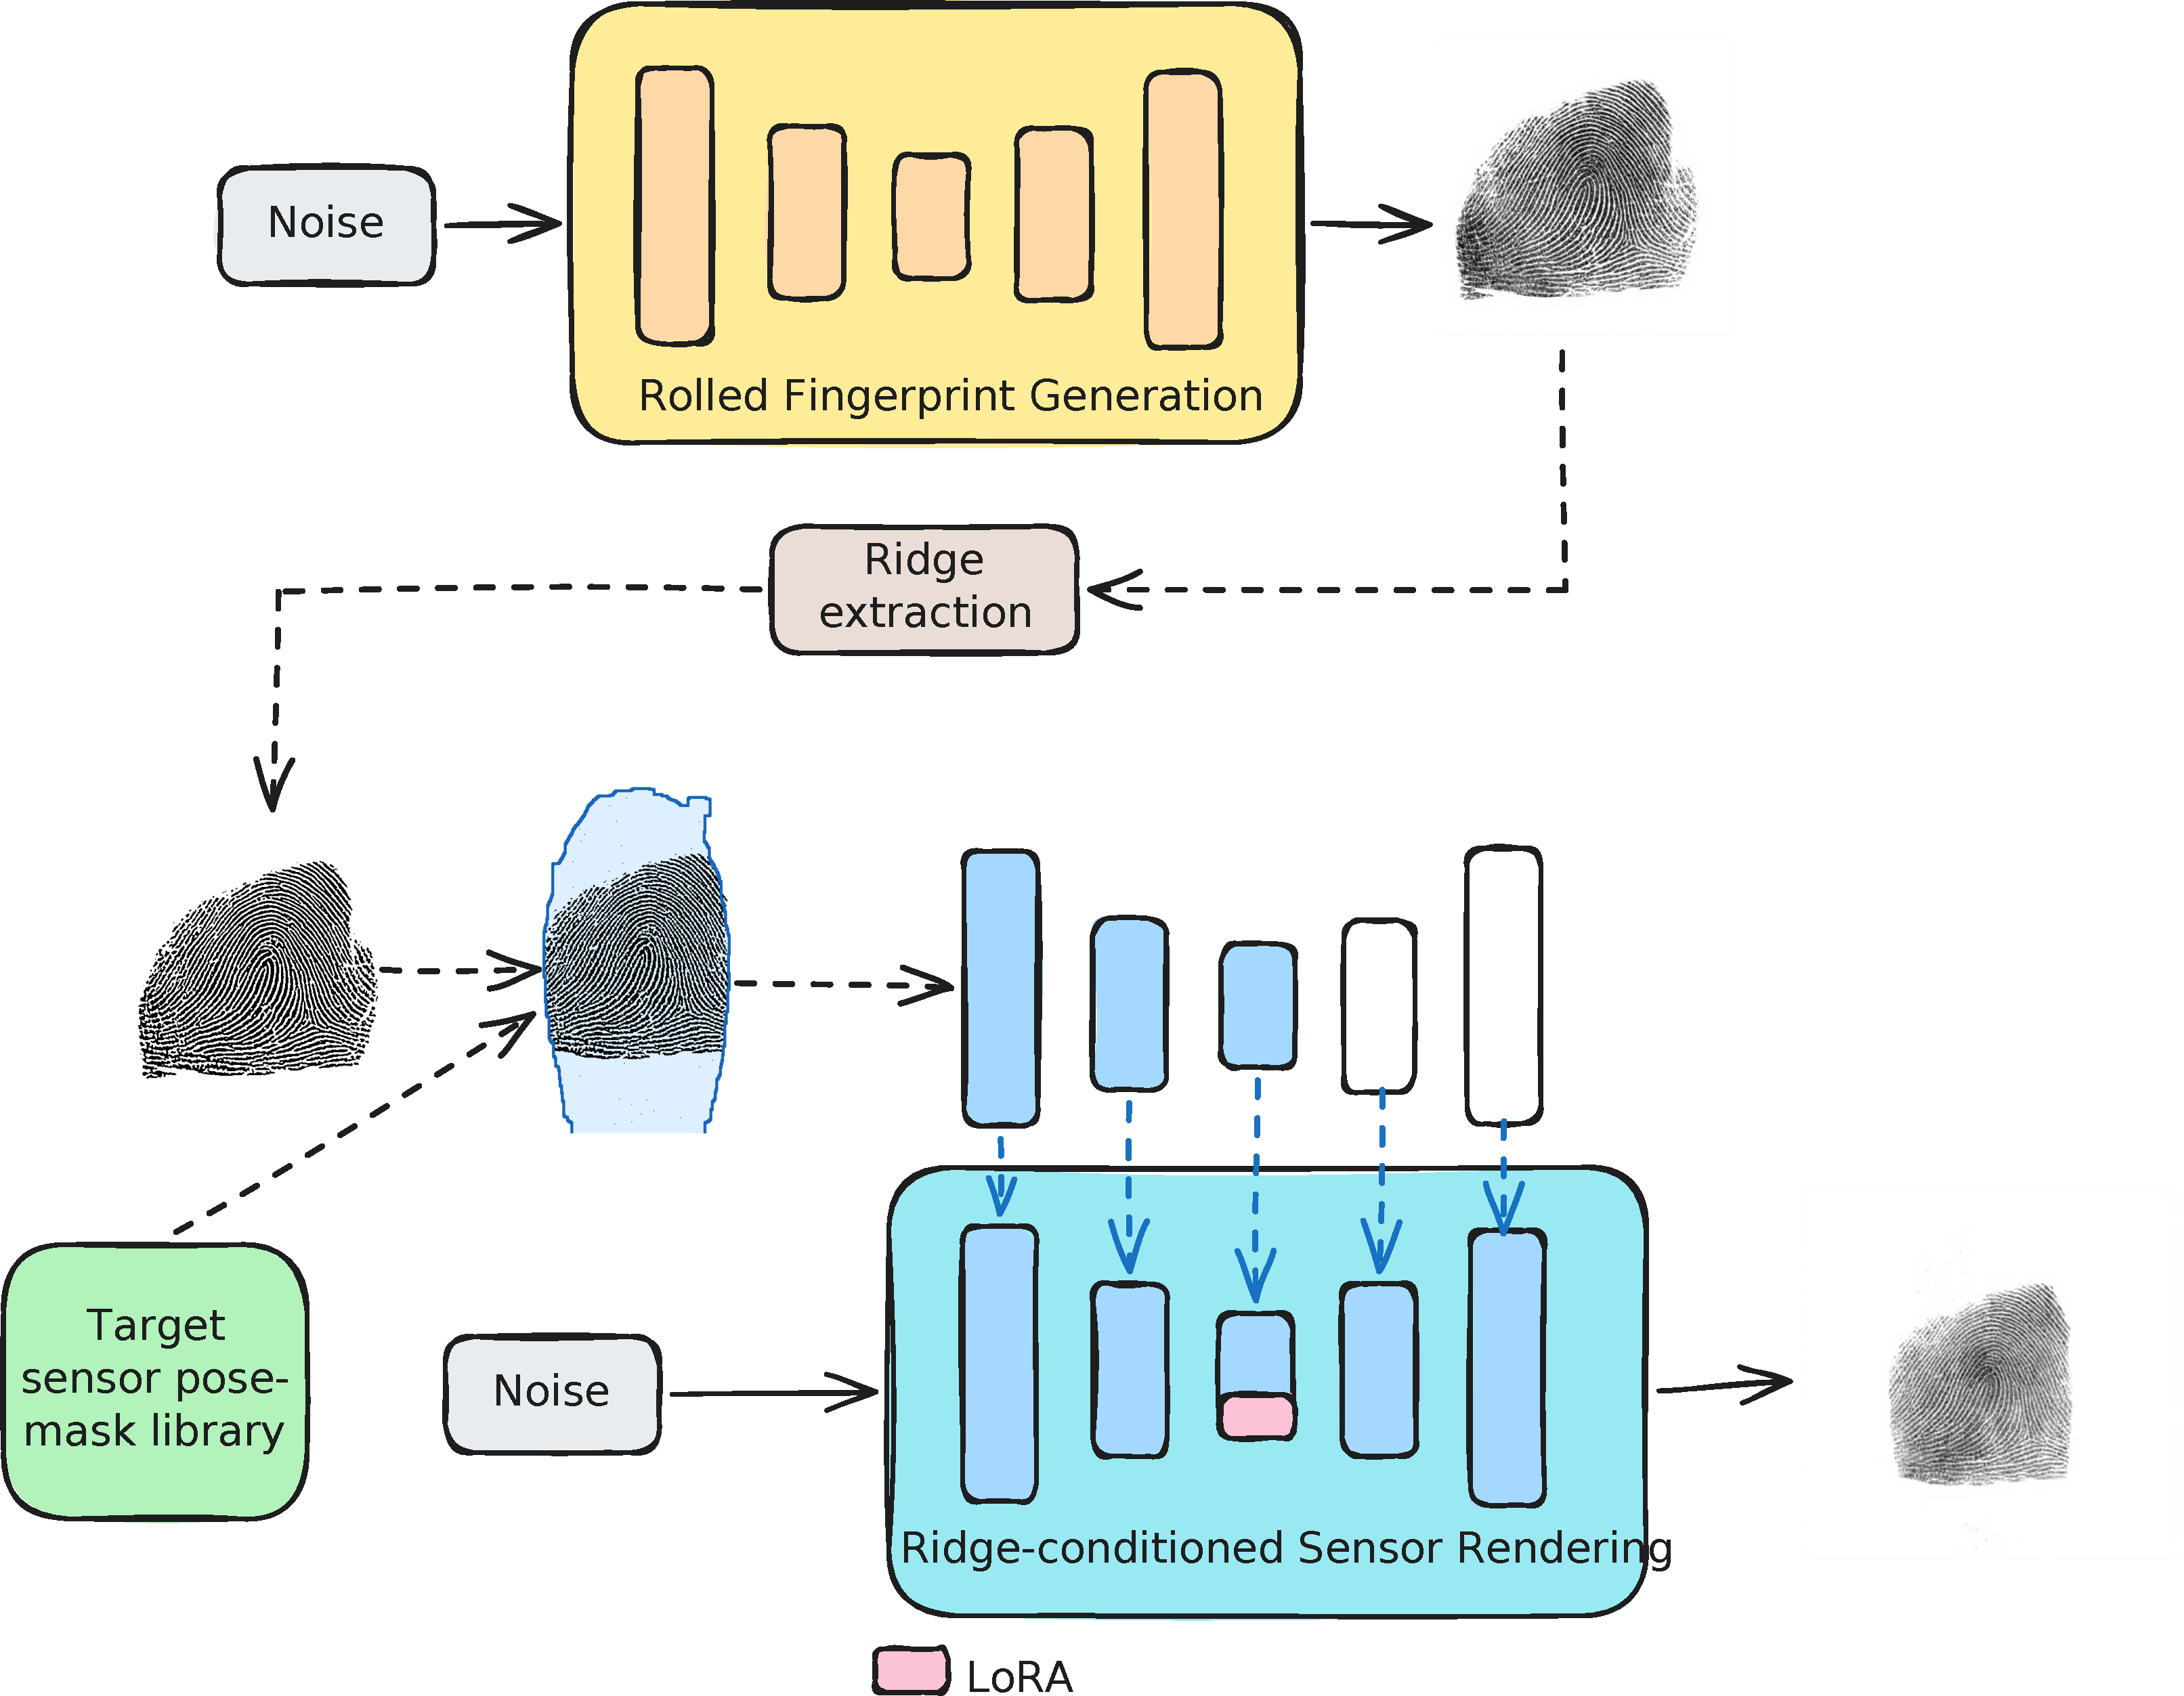
\includegraphics[width=0.98\linewidth,height=0.74\textheight,keepaspectratio]{figures/overview.pdf}
  \smallnote{Stage 1 samples a rolled identity; Stage 2 renders target-sensor
  impressions from the extracted ridge, pose mask, and selected sensor LoRA.}
\end{frame}

\begin{frame}{Stage 1: Unconditional Identity Prior}
  \begin{columns}[T,onlytextwidth]
    \begin{column}{0.45\textwidth}
      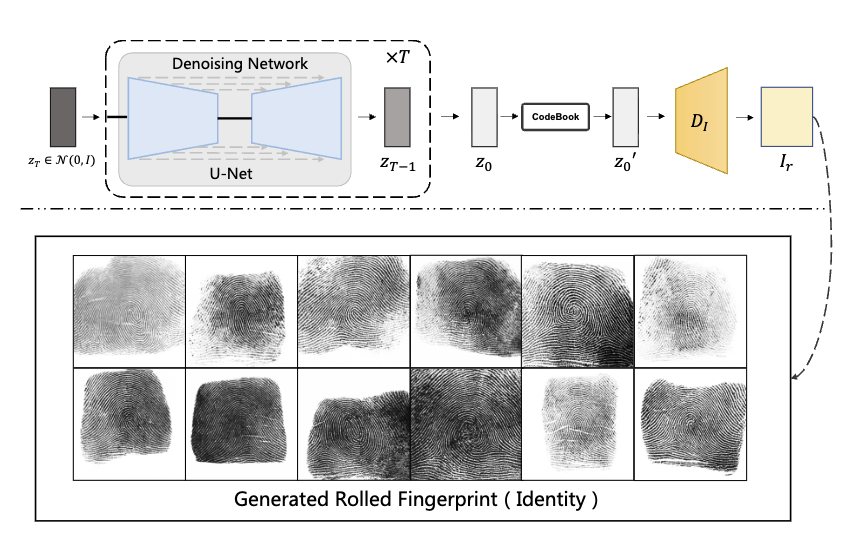
\includegraphics[width=\linewidth]{figures/stage1.png}
    \end{column}
    \begin{column}{0.52\textwidth}
      \begin{itemize}
        \item Images are encoded to frozen VQ-VAE latents:
        $512^2 \rightarrow 128 \times 128 \times 3$.
        \item Stage 1 learns an unconditional latent diffusion prior
        $p_\theta(z)$.
        \item No sensor label, text prompt, style encoder, or reference image.
        \item Output is not the final sample; it is a virtual identity used for
        ridge extraction.
      \end{itemize}
      \smallnote{High latent resolution is necessary because fingerprints are
      dominated by local, high-frequency ridge structure.}
    \end{column}
  \end{columns}
\end{frame}

\begin{frame}{Ridge Condition: Deterministic Identity Control}
  \begin{columns}[T,onlytextwidth]
    \begin{column}{0.50\textwidth}
      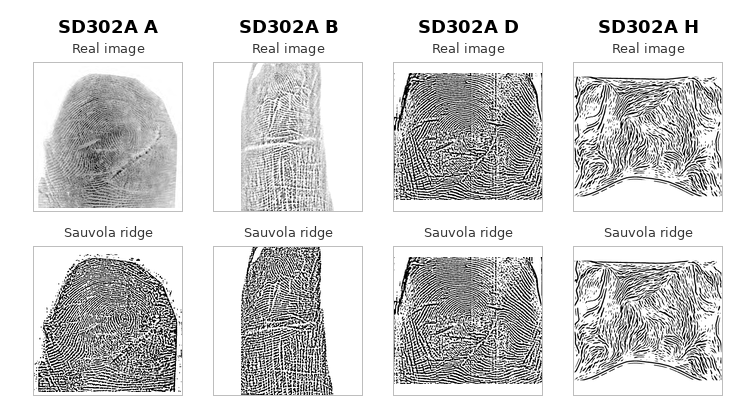
\includegraphics[width=\linewidth]{figures/sd302a_sauvola_ridge_examples.png}
    \end{column}
    \begin{column}{0.47\textwidth}
      \begin{itemize}
        \item We use Sauvola adaptive binarization:
        window $11$, $R=128$, $k=0.007$.
        \item A $2\times2$ morphological opening removes isolated noise.
        \item The binary ridge map is the identity injection signal for
        Stage 2.
        \item It avoids learned ridge hallucination and keeps the control signal
        tied to visible fingerprint texture.
      \end{itemize}
    \end{column}
  \end{columns}
\end{frame}

\begin{frame}{Pose-Mask Alignment Before Rendering}
  \begin{columns}[T,onlytextwidth]
    \begin{column}{0.56\textwidth}
      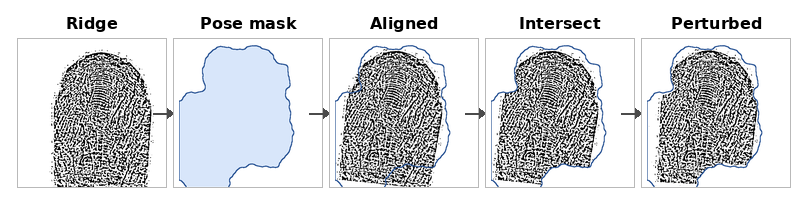
\includegraphics[width=\linewidth]{figures/pose_mask_alignment_perturbation.png}
    \end{column}
    \begin{column}{0.40\textwidth}
      \begin{itemize}
        \item Sample a target-sensor pose mask from a real mask library.
        \item Align the ridge foreground using a bounded similarity transform.
        \item Warp and clip the ridge into the target footprint.
        \item Add mild perturbations: small rotation/translation, dropout,
        speckle, light morphology.
      \end{itemize}
      \smallnote{This is what makes one identity produce multiple target-sensor
      impressions.}
    \end{column}
  \end{columns}
\end{frame}

\begin{frame}{Stage 2: Sensor Rendering with Tiny LoRA}
  \begin{columns}[T,onlytextwidth]
    \begin{column}{0.50\textwidth}
      \begin{block}{Frozen}
        VQ-VAE, Stage-1 identity prior, ridge extractor, ControlNet structural
        path, and base Stage-2 weights.
      \end{block}
      \begin{block}{Trainable per new sensor}
        Reported runs fix rank-8 LoRA on Stage-2 UNet middle self-attention
        $qkv$ and output projection due to time/resource constraints.
      \end{block}
    \end{column}
    \begin{column}{0.47\textwidth}
      \begin{itemize}
        \item Fixed rank-8 setting: \key{12.3K parameters}.
        \item Active Stage-2 transfer path: \key{23.39M parameters}.
        \item Full two-stage generator: \key{53.58M parameters}.
        \item Purpose: adapt sensor tone/artifacts without editing ridge-control
        structure.
      \end{itemize}
      \smallnote{LoRA is intentionally not placed on ControlNet because that
      would adapt the structural ridge path.}
    \end{column}
  \end{columns}
\end{frame}

\begin{frame}{LoRA Rank: Sensor-Specific Capacity}
  \begin{columns}[T,onlytextwidth]
    \begin{column}{0.48\textwidth}
      \begin{block}{Capacity}
        For the selected middle attention block,
        \[
          P(k)=1536k
        \]
      \end{block}
      \begin{itemize}
        \item Rank controls how many sensor-style directions can be learned.
        \item Rank 1/2/4/8 means 1.5K/3.1K/6.1K/12.3K trainable parameters.
        \item Available rank-8 checkpoints give a preliminary capacity hint.
        \item Final choice comes from retraining and DB\emph{x}\_B recognition.
      \end{itemize}
    \end{column}
    \begin{column}{0.49\textwidth}
      \resizebox{\linewidth}{!}{%
        \begin{tabular}{lcccc}
          \toprule
          Sensor & $k_{.90}$ & $k_{.95}$ & $k_{.99}$ & Params at $k_{.95}$ \\
          \midrule
          DB1 & 1 & 2 & 3 & 3.1K \\
          DB2 & 1 & 2 & 4 & 3.1K \\
          DB3 & 1 & 1 & 3 & 1.5K \\
          DB4 & 2 & 2 & 4 & 3.1K \\
          \bottomrule
        \end{tabular}}
      \vspace{0.65em}
      \[
        \begin{gathered}
        k_s=\text{smallest }k\\[-0.2em]
        \mathrm{TAR}_s(k)\ge \mathrm{TAR}_{s,\mathrm{best}}-\epsilon
        \end{gathered}
      \]
      \smallnote{If ranks tie, choose the smaller one. Reject a rank first if
      ridge/pose QC or LightGlue structure clearly degrades.}
    \end{column}
  \end{columns}
\end{frame}

\begin{frame}{Experimental Protocol}
  \begin{columns}[T,onlytextwidth]
    \begin{column}{0.49\textwidth}
      \begin{block}{SD302A benchmark}
        \begin{itemize}
          \item 1,600 train identities, 400 held-out identities.
          \item 10,896 real train images; 2,734 held-out test images.
          \item Synthetic set: 2,000 identities $\times$ 10 impressions.
          \item Evaluate ResNet18, ResNet50, ViT with TAR@FAR=0.1\%.
        \end{itemize}
      \end{block}
    \end{column}
    \begin{column}{0.49\textwidth}
      \begin{block}{FVC 2004 transfer}
        \begin{itemize}
          \item DB1--DB4, train adapter on only 80 DB\emph{x}\_A images.
          \item Evaluate recognition on DB\emph{x}\_B only.
          \item Synthetic set: 500 identities $\times$ 10 impressions per DB.
          \item Same ridge-mask rendering interface; select DB-specific LoRA.
        \end{itemize}
      \end{block}
    \end{column}
  \end{columns}
\end{frame}

\begin{frame}{Result 1: SD302A Recognition Utility}
  \centering
  \resizebox{0.88\linewidth}{!}{%
    \begin{tabular}{lccc}
      \toprule
      & \multicolumn{3}{c}{TAR@FAR=0.1\%} \\
      \cmidrule(lr){2-4}
      Training dataset & ResNet18 & ResNet50 & ViT \\
      \midrule
      NIST SD 302 real & 0.6946 & 0.7132 & \textbf{0.8008} \\
      FPGAN-Control & 0.7181 & 0.6626 & 0.7875 \\
      PrintsGAN & 0.5421 & 0.4561 & 0.5523 \\
      Ours & \textbf{0.7251} & \textbf{0.7251} & 0.7531 \\
      \midrule
      Real + FPGAN-Control & 0.8093 & \textbf{0.8957} & 0.8935 \\
      Real + PrintsGAN & 0.7299 & 0.7337 & 0.7688 \\
      Real + Ours & \textbf{0.8575} & 0.8938 & \textbf{0.9128} \\
      \bottomrule
    \end{tabular}}
  \vspace{0.8em}
  \begin{itemize}
    \item Synthetic-only is competitive with the strongest baseline.
    \item Real + synthetic gives the strongest ResNet18 and ViT performance.
  \end{itemize}
\end{frame}

\begin{frame}{Result 2: SD302A to FVC DB1 Transfer}
  \centering
  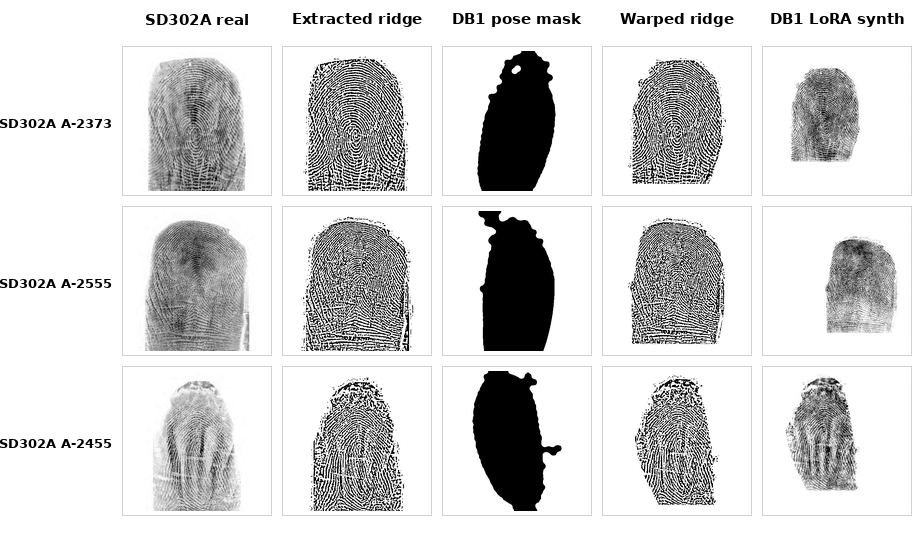
\includegraphics[width=0.95\linewidth,height=0.73\textheight,keepaspectratio]{figures/sd302a_to_fvc_db1_lora_overview.png}
  \smallnote{Pipeline: real SD302A ridge $\rightarrow$ DB1 target pose mask
  $\rightarrow$ warped/clipped ridge $\rightarrow$ Stage-2 DB1 LoRA rendering.}
\end{frame}

\begin{frame}{Result 3: FVC 2004 Cross-Sensor Recognition}
  \centering
  \resizebox{0.78\linewidth}{!}{%
    \begin{tabular}{lcccc}
      \toprule
      & \multicolumn{4}{c}{ResNet50 TAR@FAR=0.1\%} \\
      \cmidrule(lr){2-5}
      Training dataset & DB1 & DB2 & DB3 & DB4 \\
      \midrule
      DB\emph{x}\_A real & 0.7345 & 0.6905 & 0.8912 & 0.7843 \\
      Ours & 0.7530 & 0.6784 & 0.9027 & 0.7823 \\
      \midrule
      DB\emph{x}\_A real + Ours & \textbf{0.8421} & \textbf{0.7469} &
      \textbf{0.9509} & \textbf{0.8710} \\
      \bottomrule
    \end{tabular}}
  \vspace{0.8em}
  \begin{itemize}
    \item LoRA is fit from only 80 DB\emph{x}\_A images.
    \item Real + synthetic improves all four DB\emph{x}\_B evaluations.
    \item DB2 is the hardest case: low ridge/valley contrast limits synthetic-only utility.
  \end{itemize}
\end{frame}

\begin{frame}{Diagnostic: Paired Ridge Structure Is Preserved}
  \begin{columns}[T,onlytextwidth]
    \begin{column}{0.54\textwidth}
      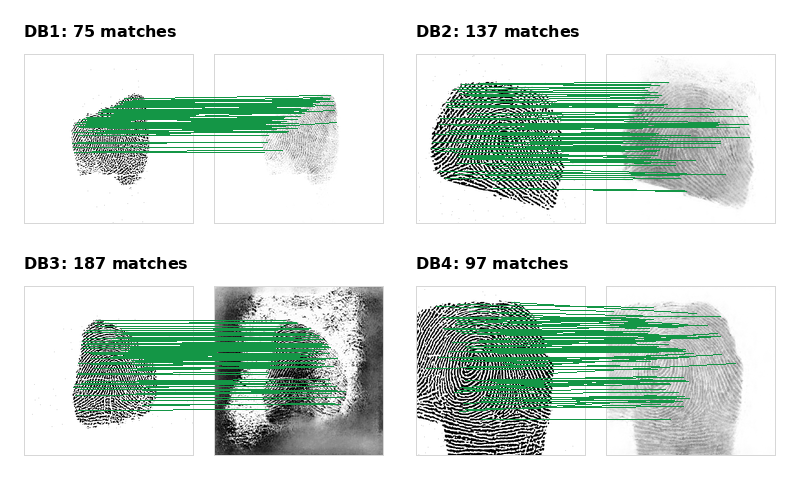
\includegraphics[width=\linewidth]{figures/lightglue_fvc_lora_matching.png}
    \end{column}
    \begin{column}{0.43\textwidth}
      \resizebox{\linewidth}{!}{%
        \begin{tabular}{lccc}
          \toprule
          Adapter & Mean matches & Median & Conf. \\
          \midrule
          DB1 & 126.2 & 84.0 & 0.319 \\
          DB2 & 123.5 & 140.5 & 0.365 \\
          DB3 & \textbf{158.7} & \textbf{185.0} & \textbf{0.420} \\
          DB4 & 99.9 & 101.0 & 0.356 \\
          \bottomrule
        \end{tabular}}
      \vspace{0.8em}
      \begin{itemize}
        \item SIFT-LightGlue matches ridge hint to rendered output.
        \item This is a paired structure diagnostic, not a biometric matcher.
      \end{itemize}
    \end{column}
  \end{columns}
\end{frame}

\begin{frame}{Diagnostic: DB-Specific Sensor Styles}
  \begin{columns}[T,onlytextwidth]
    \begin{column}{0.54\textwidth}
      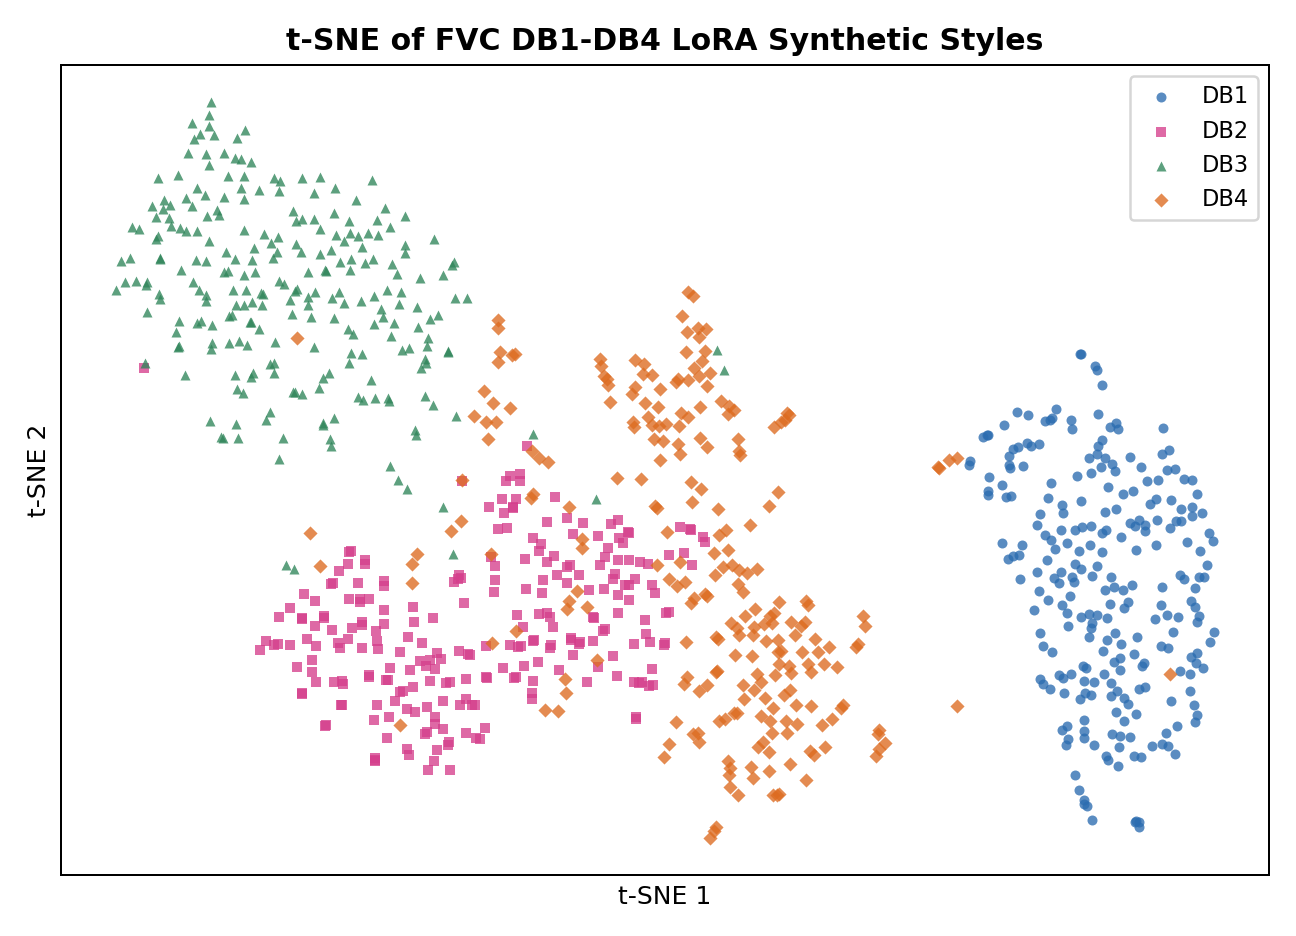
\includegraphics[width=\linewidth]{figures/fvc_lora_tsne.png}
    \end{column}
    \begin{column}{0.43\textwidth}
      \begin{itemize}
        \item 250 shared synthetic filenames per adapter, 1,000 images total.
        \item Descriptor: thumbnails, foreground masks, local contrast, intensity
        histograms, global statistics.
        \item 2D t-SNE silhouette: \key{0.446}.
        \item DB1 separates most cleanly; DB2 and DB4 are closer.
      \end{itemize}
    \end{column}
  \end{columns}
\end{frame}

\begin{frame}{Ablations: What Actually Matters?}
  \begin{columns}[T,onlytextwidth]
    \begin{column}{0.50\textwidth}
      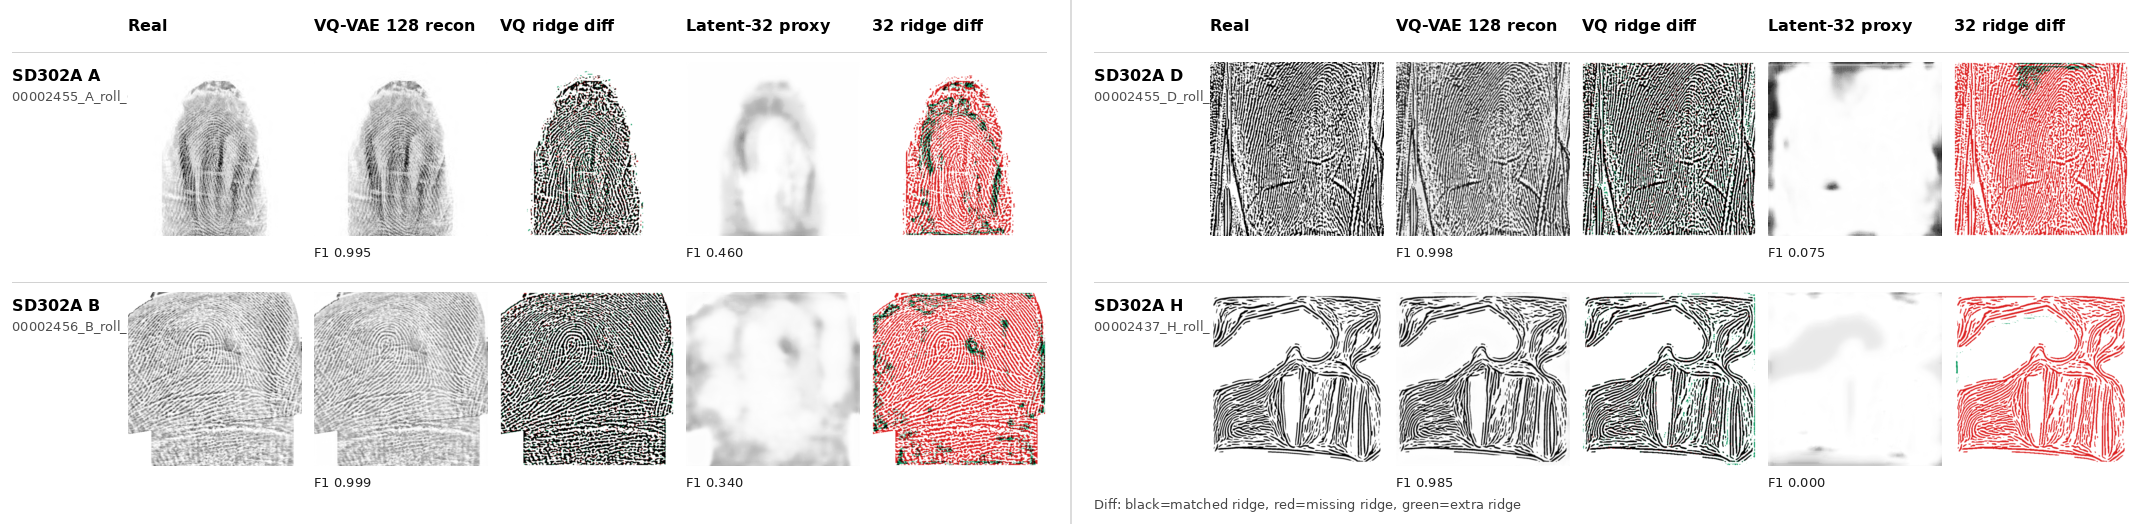
\includegraphics[width=\linewidth]{figures/ablation_vqvae128_vs_latent32_wide.png}
      \smallnote{$128^2$ latent preserves ridge topology; $32^2$ proxy blurs it.}
    \end{column}
    \begin{column}{0.47\textwidth}
      \begin{block}{Key ablation numbers}
        \begin{itemize}
          \item $128^2$ latent: ridge F1 = 0.994 at 2 px tolerance.
          \item $32^2$ proxy: ridge F1 = 0.219 at 2 px tolerance.
          \item Sauvola active foreground: 53.3\%; Canny: 28.3\%.
          \item Canny has 2.8$\times$ more fragmented control support.
          \item Rank capacity: DB3 reaches 95\% update energy at rank 1;
          DB1/DB2/DB4 need rank 2, and DB2/DB4 need rank 4 at 99\%.
        \end{itemize}
      \end{block}
    \end{column}
  \end{columns}
\end{frame}

\begin{frame}{Efficiency and Practicality}
  \centering
  \resizebox{0.80\linewidth}{!}{%
    \begin{tabular}{lrlr}
      \toprule
      Component & Params & Component & Params \\
      \midrule
      Stage-1 identity UNet & 16.33M & Stage-2 denoising UNet & 16.35M \\
      Stage-2 ControlNet & 7.04M & VQ-VAE encoder/decoder/codebook & 13.86M \\
      Full two-stage generator & 53.58M & Active Stage-2 path & 23.39M \\
      \midrule
      Fixed rank-8 LoRA / sensor & \textbf{12.3K} & Logged generation & 1.05 s/image \\
      \bottomrule
    \end{tabular}}
  \vspace{0.9em}
  \begin{itemize}
    \item Active Stage-2 transfer path is 97.3--98.5\% smaller than SD1-style
    UNet/ControlNet-scale pipelines.
    \item New sensor adaptation trains only LoRA; rank can be chosen per sensor.
  \end{itemize}
\end{frame}

\begin{frame}{Limitations}
  \begin{itemize}
    \item Stage 2 inherits errors from ridge extraction and pose-mask alignment;
    warping/clipping can remove minutiae-scale evidence.
    \item Reported recognition runs fix rank-8 LoRA for all FVC sensors due to
    time/resource constraints; a retraining sweep is needed to choose ranks.
    \item LightGlue and t-SNE are supporting diagnostics, not full biometric
    validation.
    \item Future work: minutiae-aware losses, better foreground masks,
    quality-aware adapter capacity, and larger cross-sensor protocols.
  \end{itemize}
\end{frame}

\begin{frame}{Takeaways}
  \begin{block}{Main result}
    \method{} separates identity generation from sensor rendering and adapts to
    unseen sensor styles with a small, sensor-specific LoRA adapter.
  \end{block}
  \begin{itemize}
    \item Explicit ridge conditioning keeps identity evidence under control.
    \item Target pose masks and perturbations add impression-level variation.
    \item Real + synthetic consistently improves SD302A and FVC recognition.
    \item LoRA rank should be selected per sensor; low-contrast sensors remain
    the main failure mode.
  \end{itemize}
\end{frame}

\appendix

\begin{frame}{Backup: Sauvola vs. Canny Control}
  \begin{columns}[T,onlytextwidth]
    \begin{column}{0.50\textwidth}
      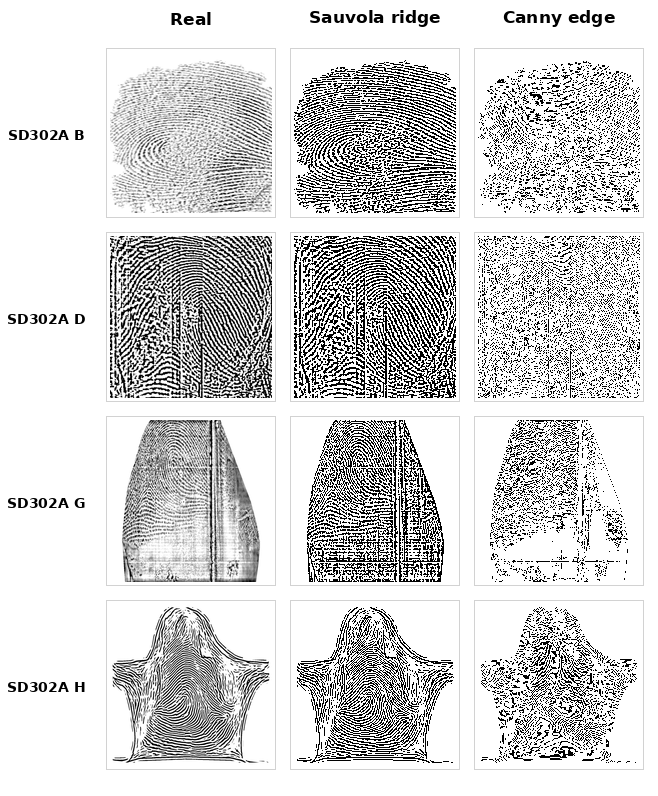
\includegraphics[width=\linewidth,height=0.68\textheight,keepaspectratio]{figures/ablation_sauvola_vs_canny.png}
    \end{column}
    \begin{column}{0.47\textwidth}
      \resizebox{\linewidth}{!}{%
        \begin{tabular}{lcccc}
          \toprule
          Control & Active fg. & 3x3 support & Comp./10k & Largest comp. \\
          \midrule
          Sauvola & 53.3 & 33.1 & 83.3 & 13236.9 \\
          Canny & 28.3 & 0.0 & 230.6 & 1723.3 \\
          \bottomrule
        \end{tabular}}
      \vspace{0.8em}
      \smallnote{Canny marks contours and artifacts; Sauvola gives dense
      ridge-phase support.}
    \end{column}
  \end{columns}
\end{frame}

\begin{frame}{Backup: LoRA Placement}
  \centering
  \resizebox{0.86\linewidth}{!}{%
    \begin{tabular}{lrrl}
      \toprule
      Placement & Trainable & Rel. & Decision \\
      \midrule
      No adapter & 0 & 0.00x & Cannot adapt target sensor appearance \\
      Stage-2 mid-attn qkv only & 8.2K & 0.67x & Partial: output remix fixed \\
      Stage-2 mid-attn proj only & 4.1K & 0.33x & Partial: q/k/v fixed \\
      Stage-2 mid-attn qkv+proj & \textbf{12.3K} & \textbf{1.00x} & Selected \\
      ControlNet mid-attn qkv+proj & 12.3K & 1.00x & Rejected: edits ridge path \\
      All Stage-2 self-attn blocks & 119.8K & 9.75x & Too much for 80-image fitting \\
      Full Stage-2 UNet & 23.39M & 1903x & No longer lightweight \\
      \bottomrule
    \end{tabular}}
\end{frame}

\begin{frame}{Backup: DB2 Failure Diagnostic}
  \centering
  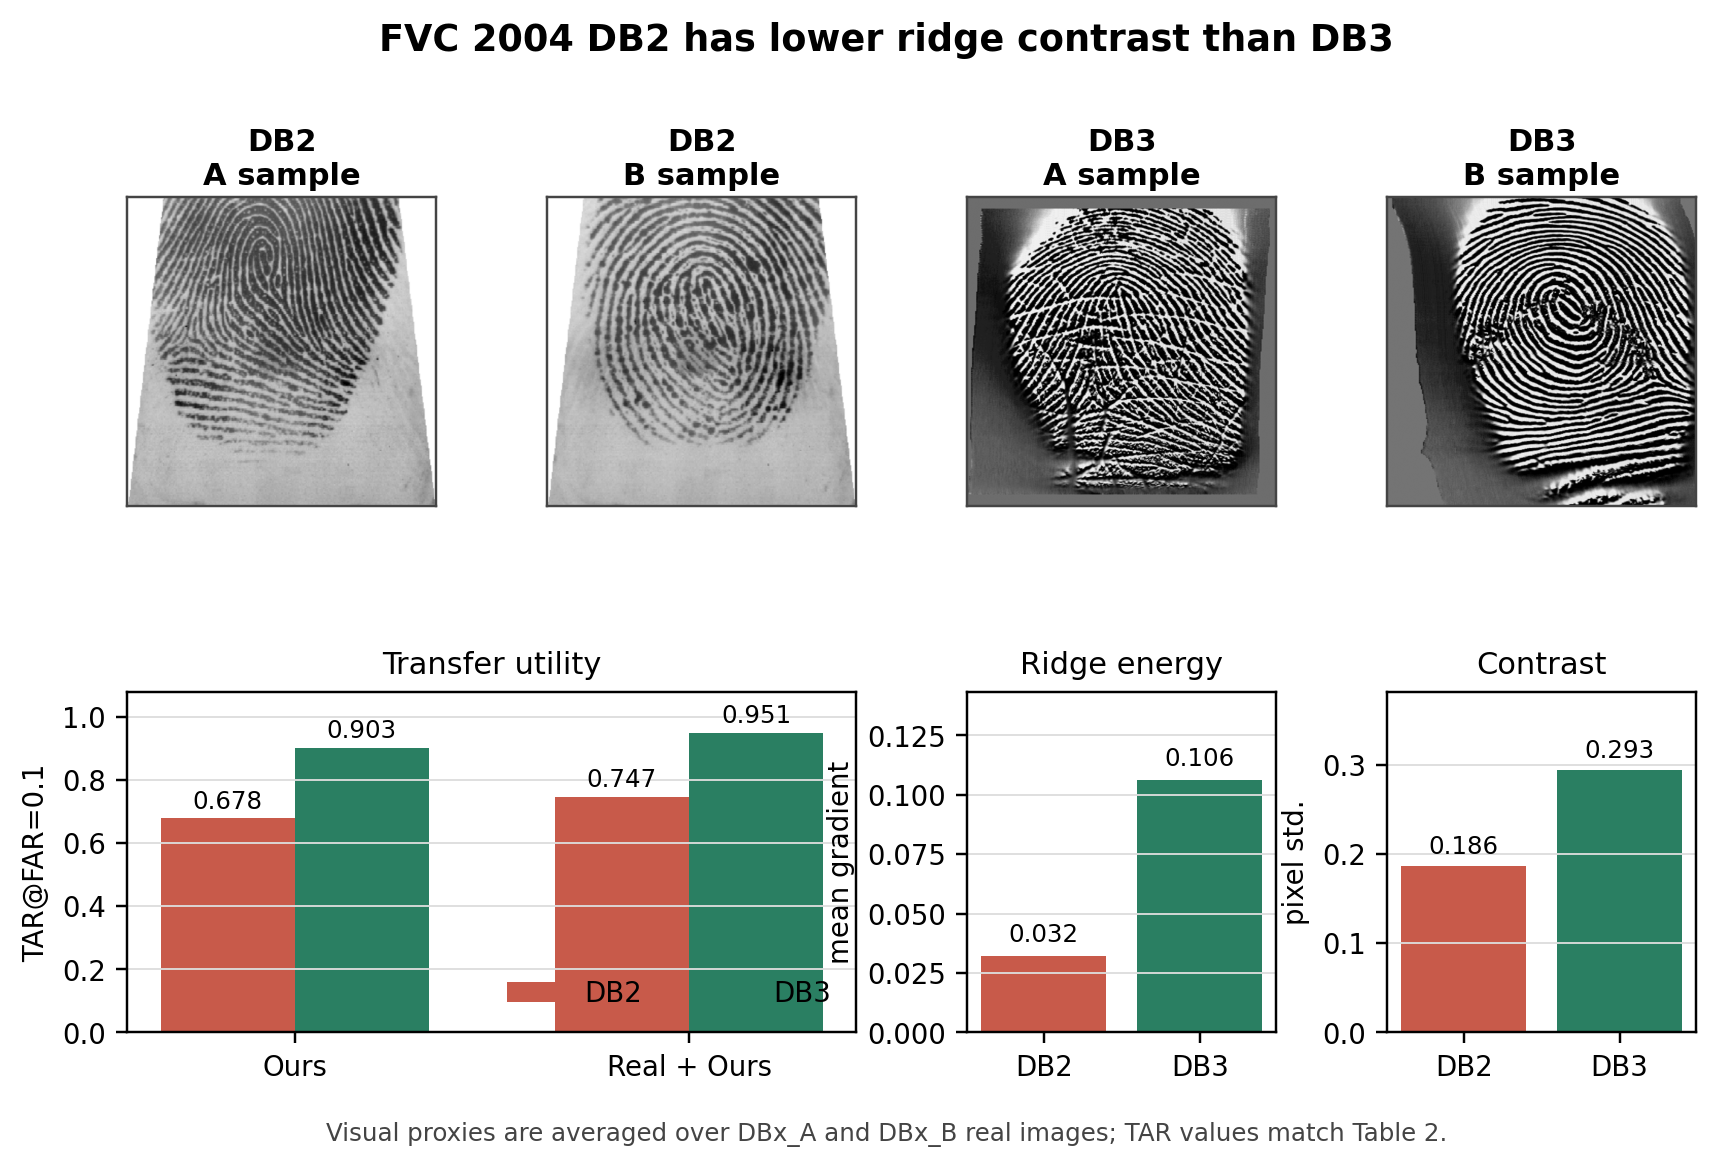
\includegraphics[width=0.84\linewidth,height=0.70\textheight,keepaspectratio]{figures/fvc_db2_db3_transfer_diagnostics.png}
  \smallnote{DB2 has weaker ridge/valley contrast than DB3, which explains the
  smaller synthetic-only and real-plus-synthetic gains.}
\end{frame}

\begin{frame}{Backup: DB1 Real vs. Synthetic Page}
  \centering
  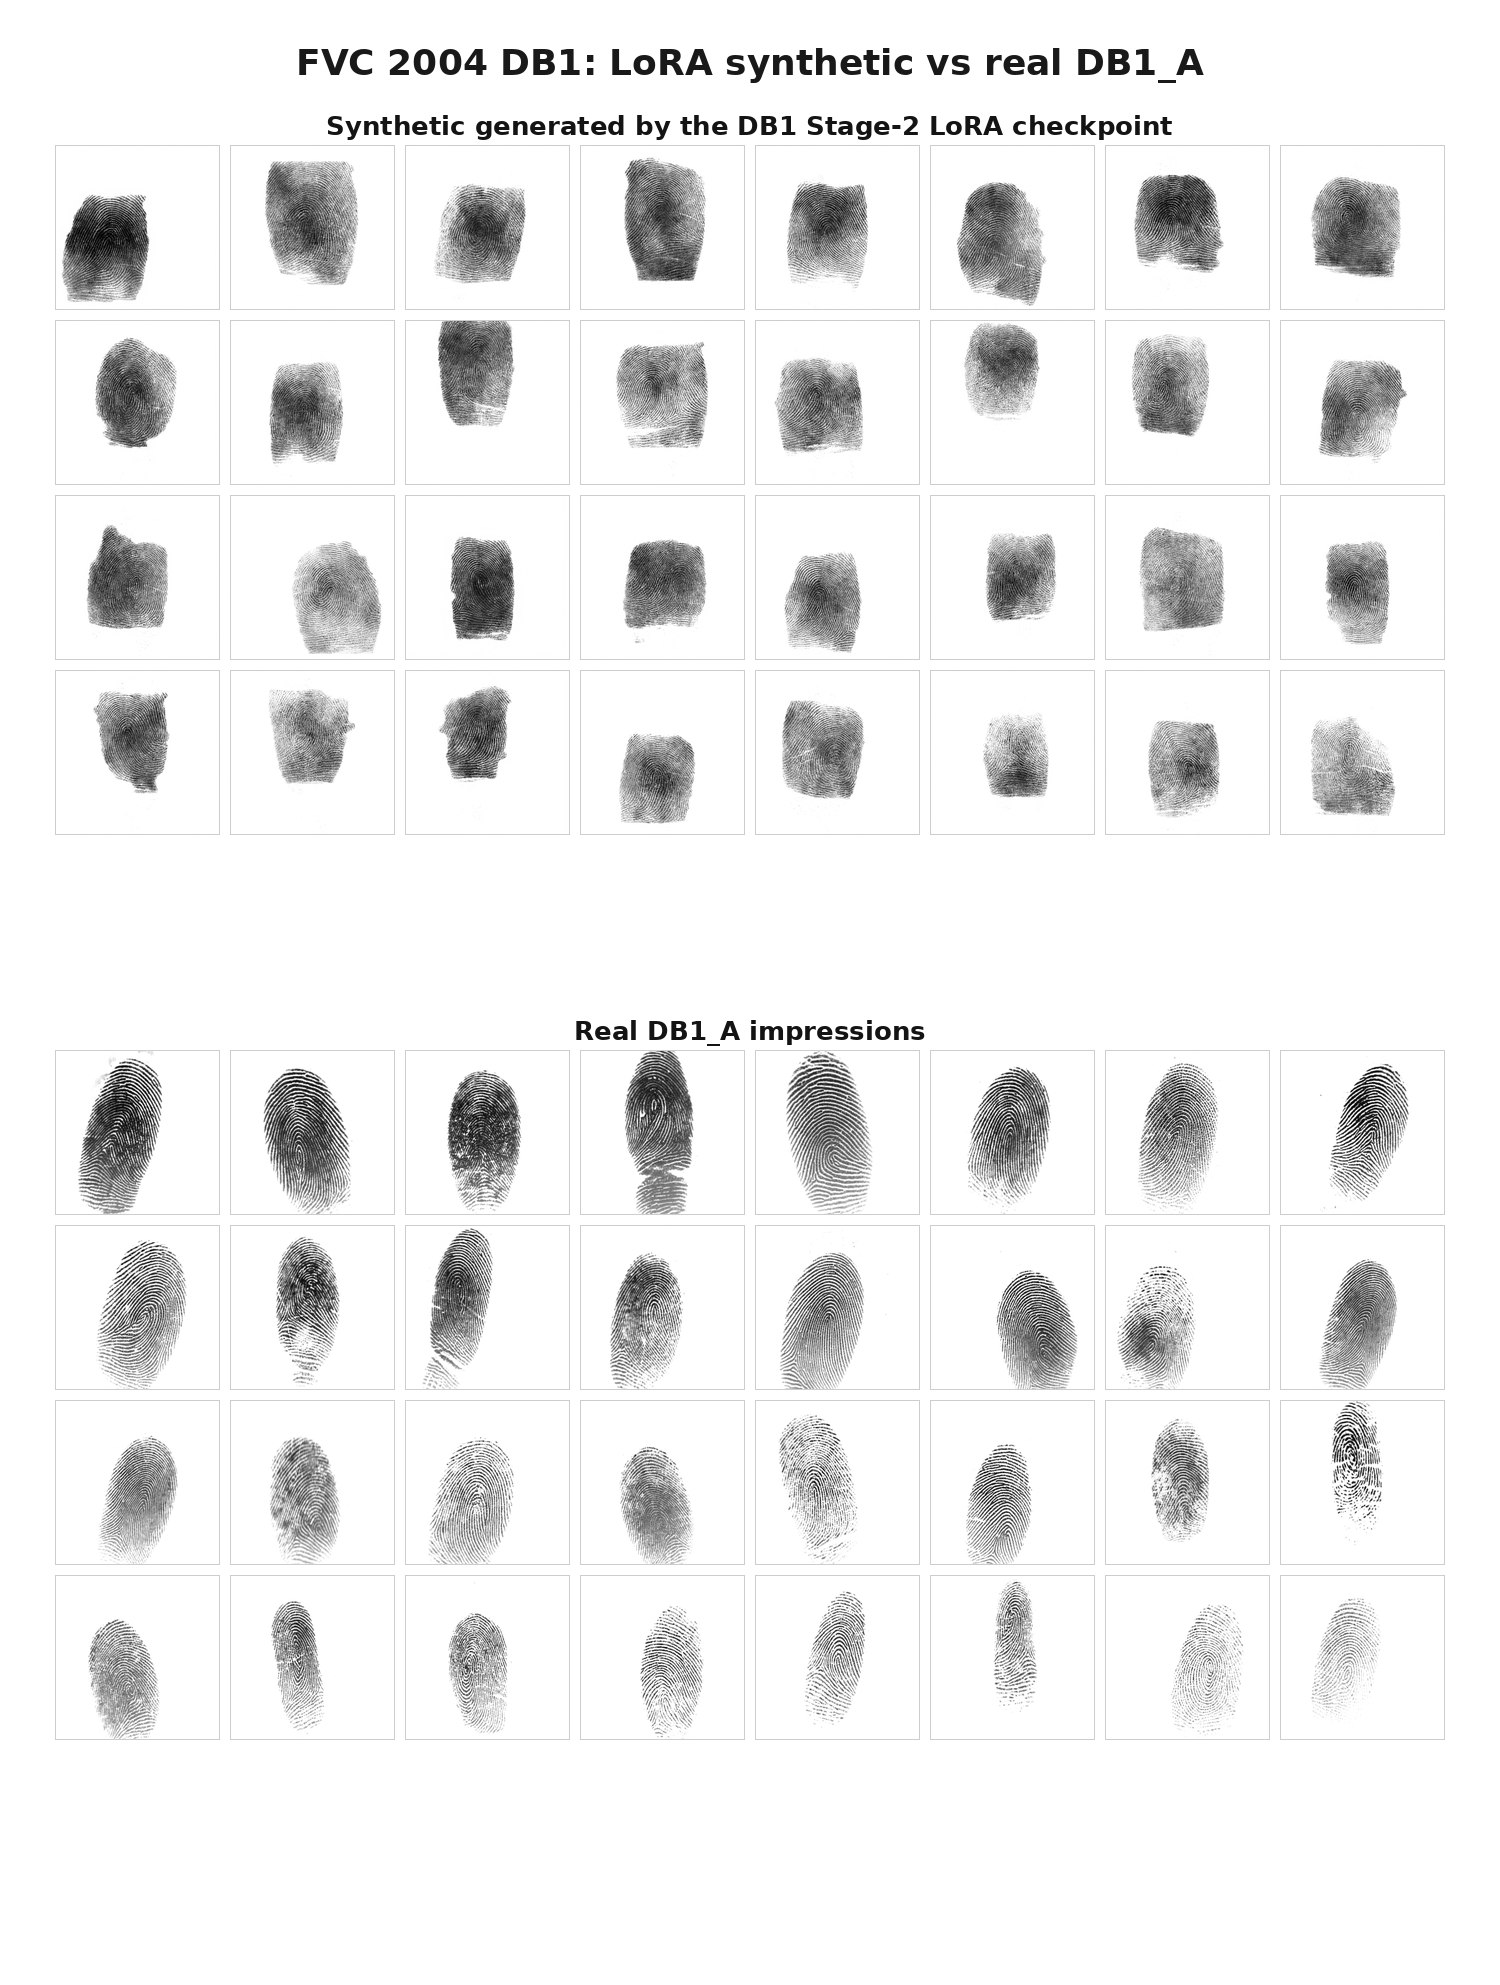
\includegraphics[width=0.82\linewidth,height=0.78\textheight,keepaspectratio]{figures/fvc_lora_db1_real_synth_page.png}
\end{frame}

\begin{frame}{Backup: DB2--DB4 Real vs. Synthetic Pages}
  \begin{columns}[T,onlytextwidth]
    \begin{column}{0.32\textwidth}
      \centering
      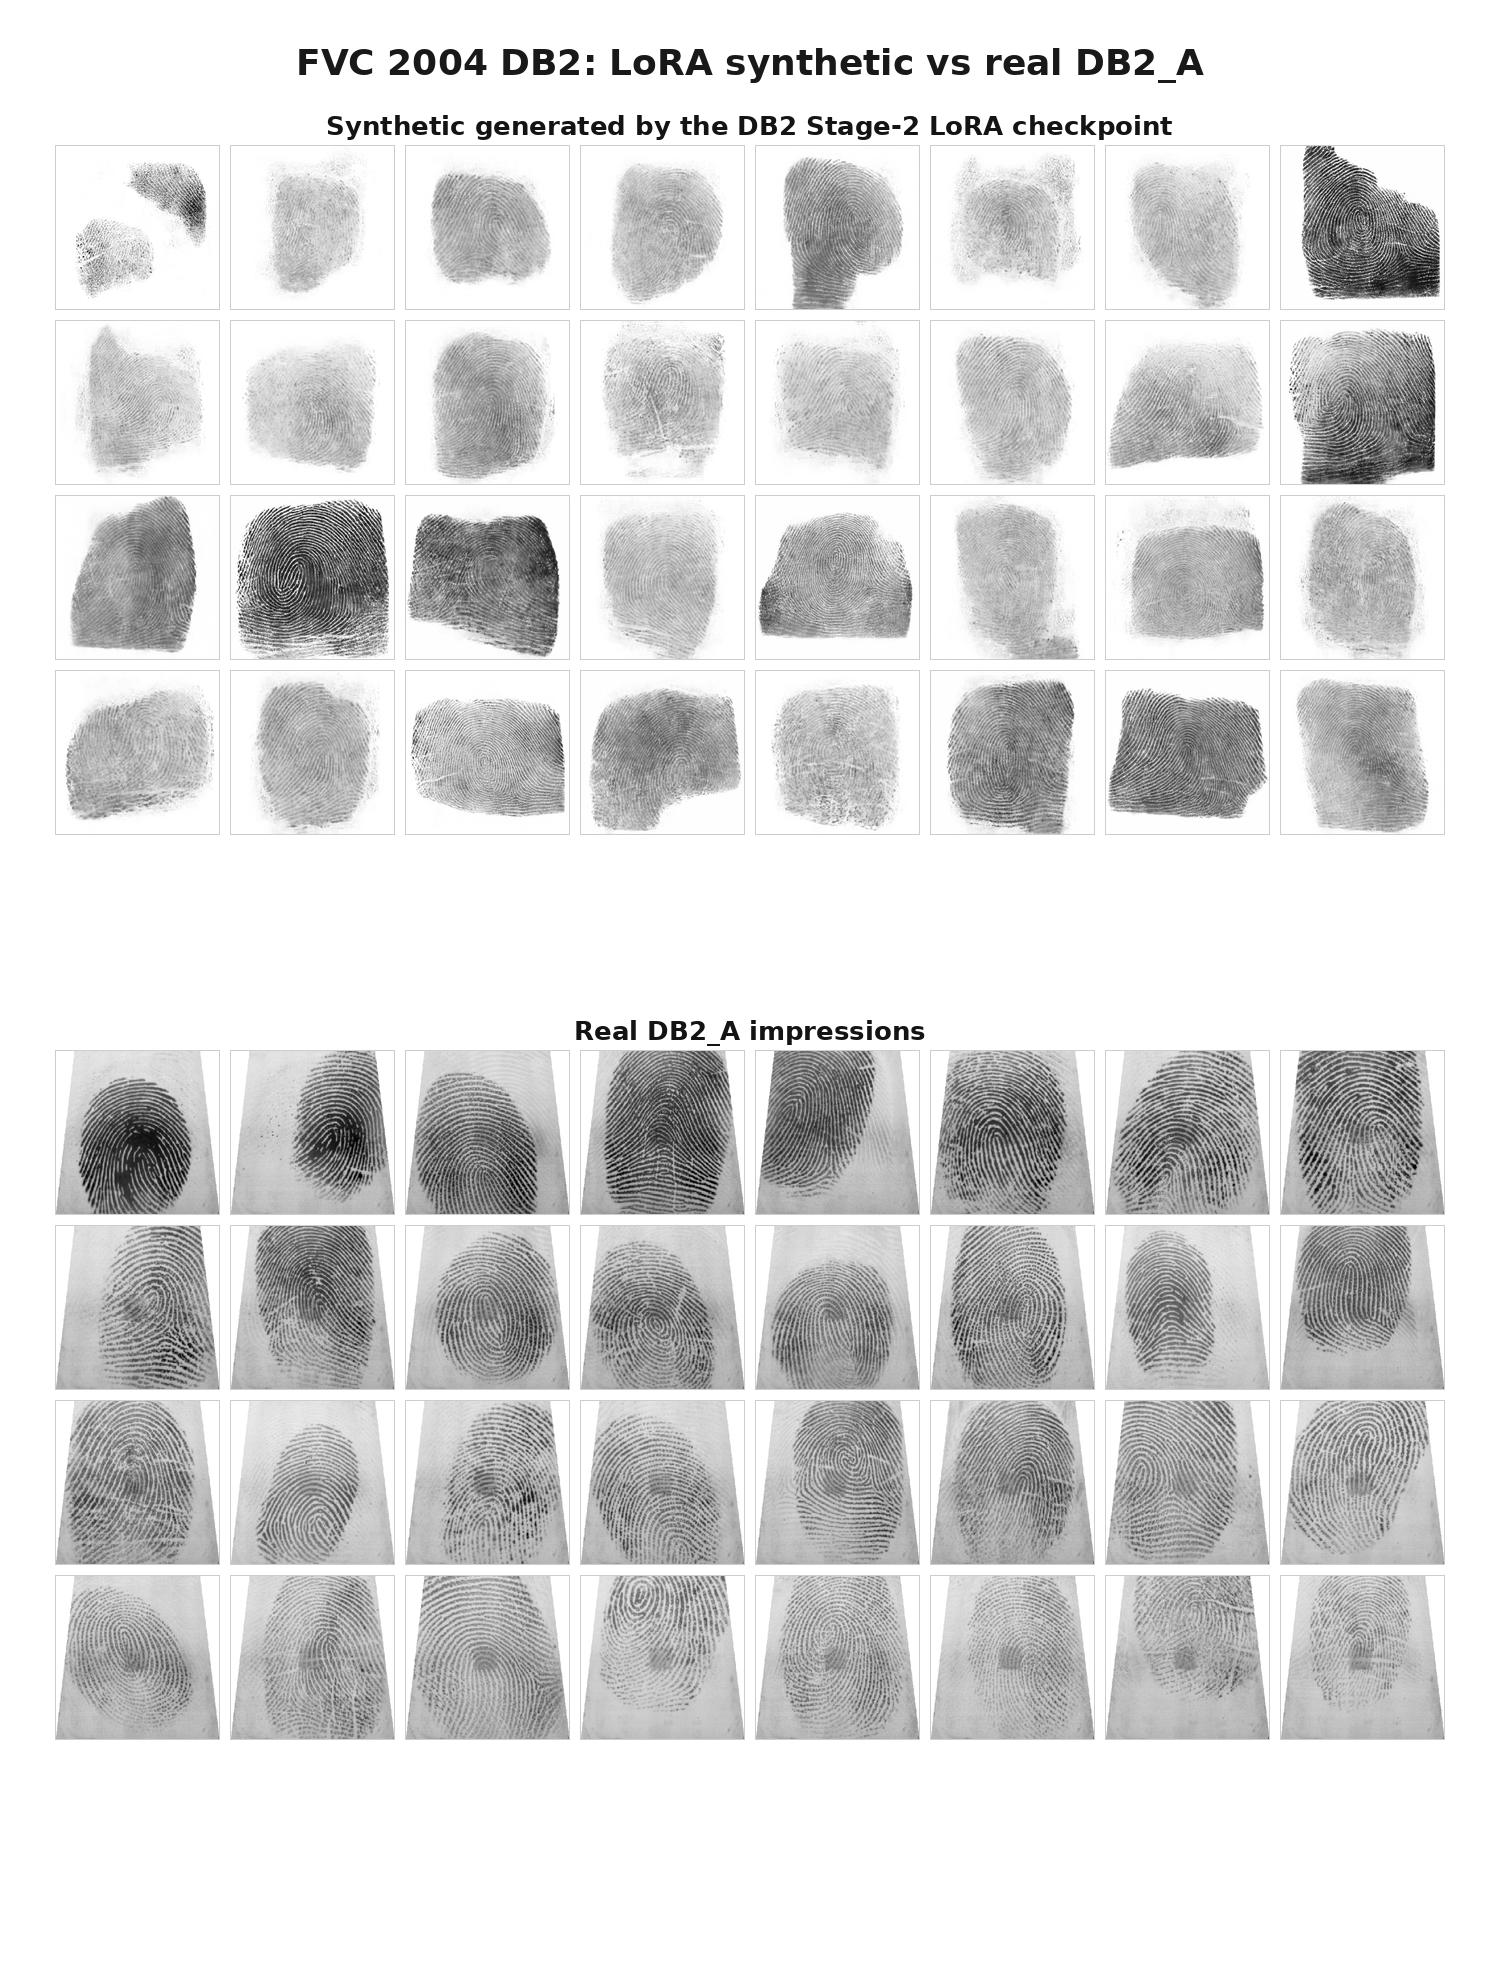
\includegraphics[width=\linewidth,height=0.72\textheight,keepaspectratio]{figures/fvc_lora_db2_real_synth_page.png}\\
      {\scriptsize DB2}
    \end{column}
    \begin{column}{0.32\textwidth}
      \centering
      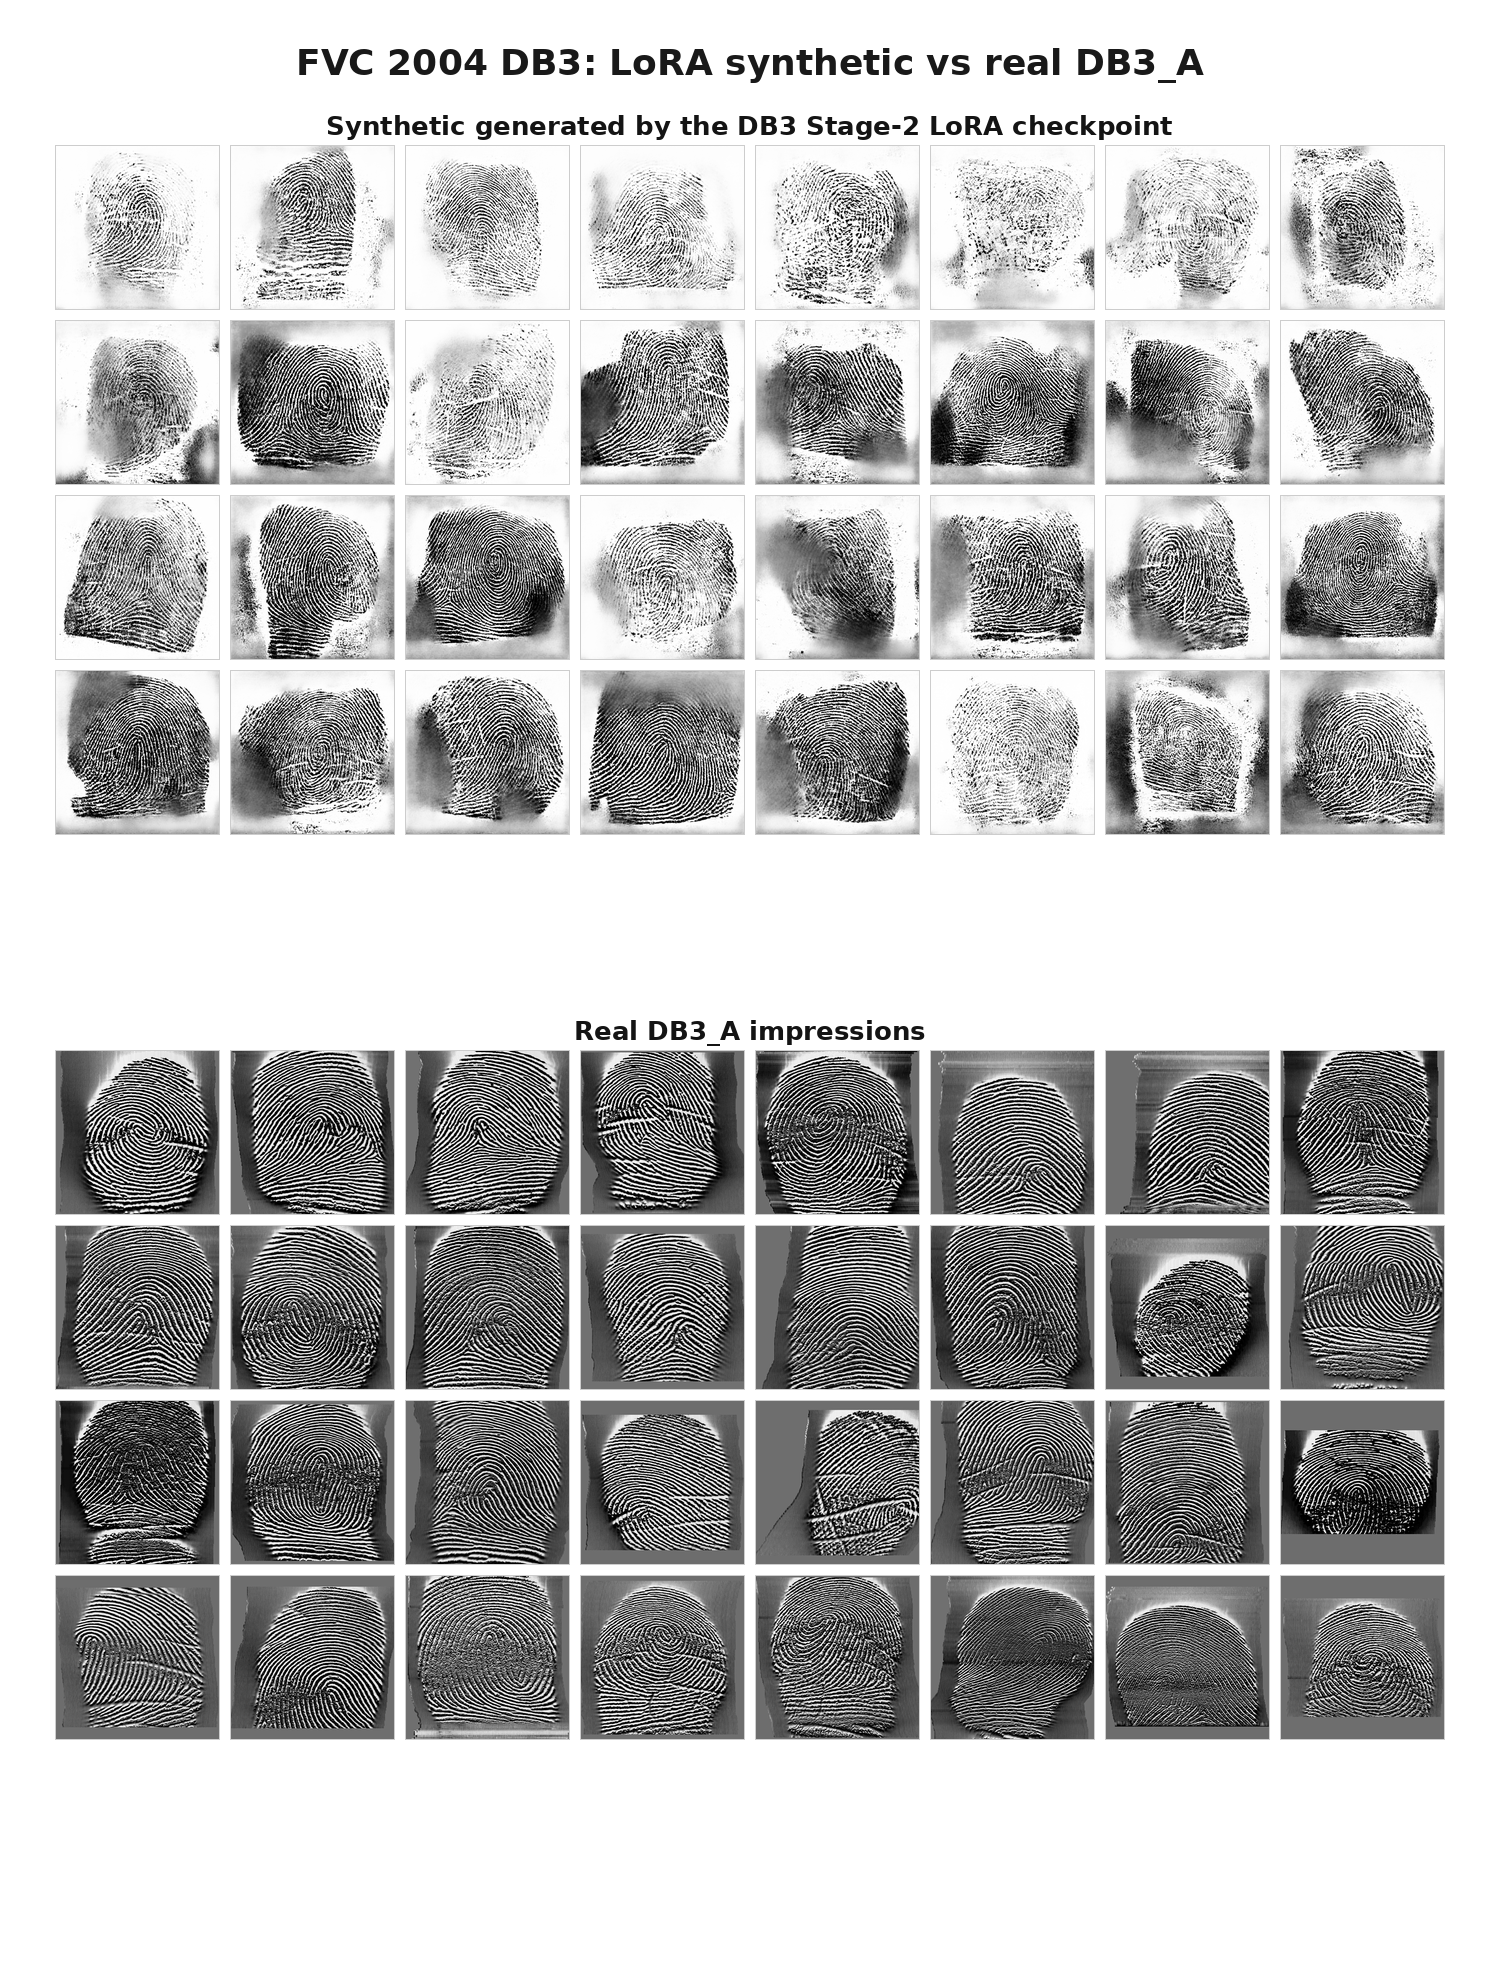
\includegraphics[width=\linewidth,height=0.72\textheight,keepaspectratio]{figures/fvc_lora_db3_real_synth_page.png}\\
      {\scriptsize DB3}
    \end{column}
    \begin{column}{0.32\textwidth}
      \centering
      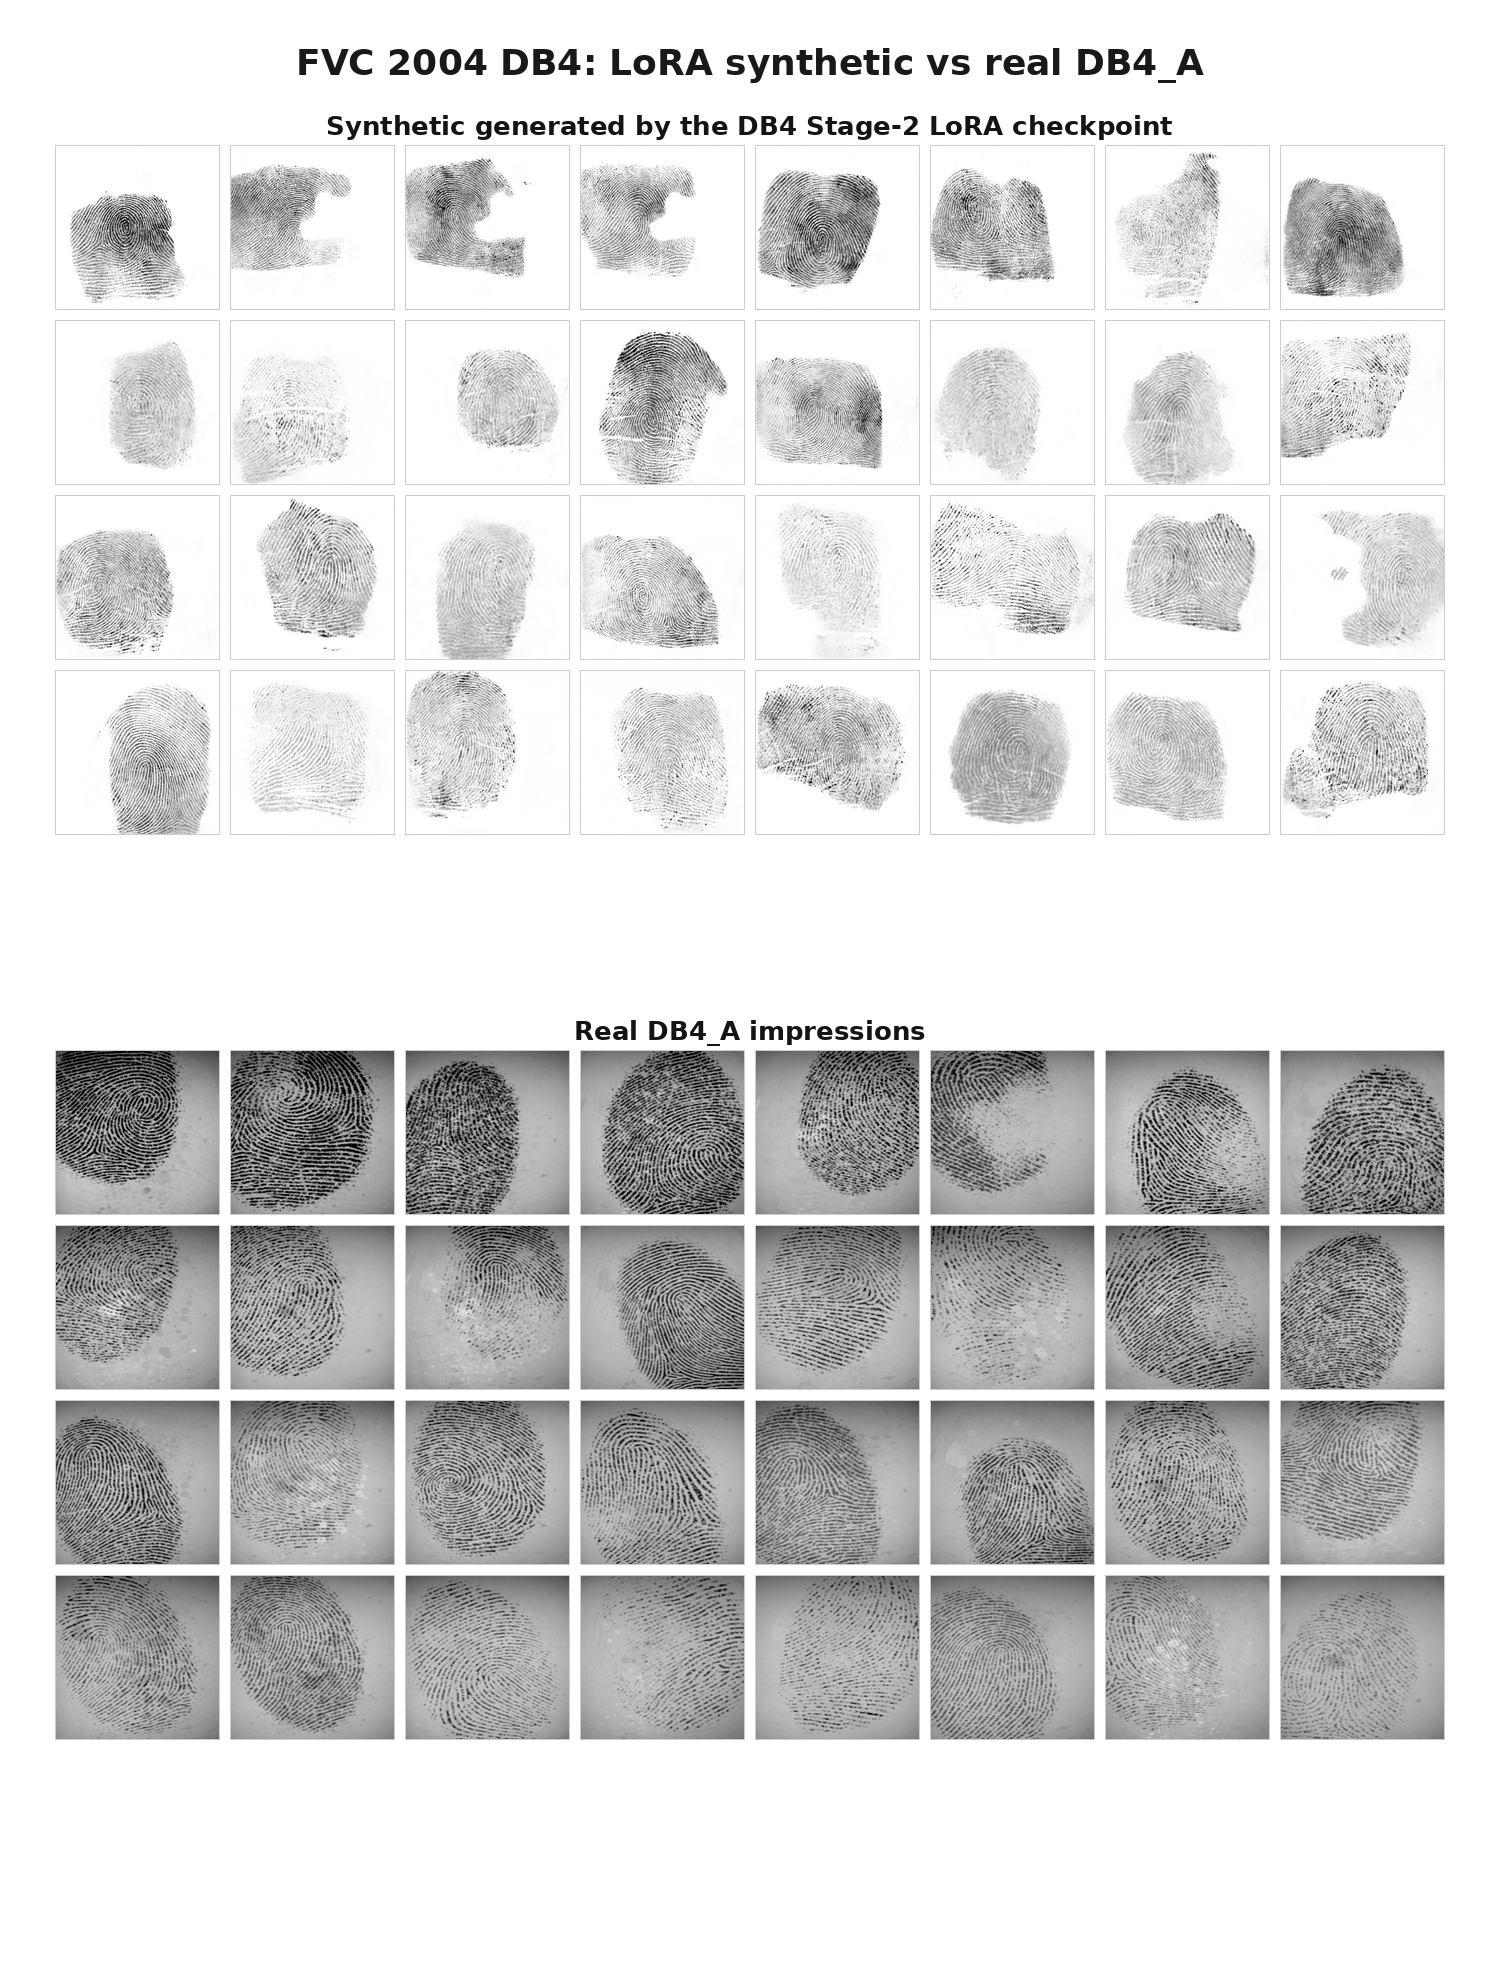
\includegraphics[width=\linewidth,height=0.72\textheight,keepaspectratio]{figures/fvc_lora_db4_real_synth_page.png}\\
      {\scriptsize DB4}
    \end{column}
  \end{columns}
\end{frame}

\end{document}
